\documentclass[11pt]{article}

\usepackage[margin=1in]{geometry}
\usepackage{amsmath, amssymb}
\usepackage{booktabs}
\usepackage{graphicx}
\usepackage{hyperref}
\usepackage{microtype}
\usepackage{enumitem}
\usepackage{tabularx}
\usepackage{array}
\usepackage{multirow}
\usepackage{natbib}

\bibliographystyle{unsrtnat}

\title{Supplementary Information\\[6pt]
\large Cognitive architecture moderates emotion--cognition relationships:
cross-domain evidence from meta-analytic reanalysis}

\author{[Author information omitted for double-blind review]}

\date{}

\begin{document}
\maketitle


\begin{table}[ht]
\centering
\small
\caption*{\textbf{Supplementary Table 1.} Specific falsifiable
predictions derived from the DLN framework for emotion--cognition
relationships. Each prediction names the specific construct, proposed
measure, and expected direction by DLN stage. Predictions are
numbered to facilitate tracking across future empirical tests.}
\begin{tabularx}{\linewidth}{p{0.03\linewidth} p{0.13\linewidth} X p{0.22\linewidth}}
\toprule
\textbf{\#} & \textbf{Construct} & \textbf{Prediction} & \textbf{Measure(s)} \\
\midrule
S1 & Emotional granularity &
Granularity increases across DLN stages: dot $<$ linear $<$ network.
Dot-stage individuals show undifferentiated affect; linear-stage
individuals show basic category distinctions; network-stage individuals
show fine-grained differentiation. &
Levels of Emotional Awareness Scale (LEAS\cite{Lane1990}); experience
sampling affect grids \\[6pt]
S2 & Alexithymia (curvilinear) &
TAS-20 scores show a curvilinear relationship with DLN stage:
\textit{highest} for linear-stage individuals (active suppression),
moderate for dot-stage (emotional opacity without suppression),
\textit{lowest} for network-stage (integration). &
Toronto Alexithymia Scale (TAS-20\cite{Bagby1994}) \\[6pt]
S3 & Decision quality under load &
Dot: impaired across load levels. Linear: intact under low load,
sharp decline under high load. Network: gradual, proportional decline.
The stage $\times$ load interaction is the key test. &
Iowa Gambling Task variants; Balloon Analogue Risk Task under affect
induction \\[6pt]
S4 & Dangerous-middle &
Individuals with relational emotional knowledge but low metacognitive
monitoring exhibit \textit{worse} outcomes under high affective load
than linear-stage compartmentalisers. This reversal is not predicted
by monotonic stage models. \textit{Supported:} Hoyt et al.\
(2024) show linear-coded domains produce significantly worse
outcomes than dot-coded domains ($b = -0.16$, 95\% CI $[-0.30,
-0.01]$). &
LEAS (relational knowledge); structural-revision tasks (monitoring);
high-load decision paradigms \\[6pt]
S5 & Implicit--explicit gaps &
Implicit--explicit attitude discrepancies are largest for linear-stage
individuals (systematic suppression) and smallest for network-stage
individuals (integration aligns implicit and explicit). Dot-stage shows
moderate discrepancy (inconsistency, not systematic suppression). &
Implicit Association Test (IAT\cite{Greenwald1998}); explicit
self-report attitude scales \\[6pt]
S6 & Recovery after disruption &
Recovery time after emotional disruption is slowest for linear-stage
(re-establishing suppression), fastest for network-stage (integrating
experience), intermediate for dot-stage (reactive dissipation). &
Affect recovery paradigms; physiological return-to-baseline measures \\
\bottomrule
\end{tabularx}
\end{table}


\subsection*{Supplementary Table 2: Coding sensitivity audit}

To assess robustness to coding ambiguity, we identified the most
debatable stage assignments in each dataset and reran all analyses
under every plausible alternative coding. For each scenario, we report
the residual $\hat\tau^2$, percentage reduction from baseline, and
whether the qualitative sign pattern is preserved. Across all 47
scenarios (16 DLN-stage and 31 Greenwald topology) the qualitative
pattern was preserved in every case (47/47, 100\%). Among the 16
DLN-stage scenarios, $\hat\tau^2$ reduction exceeded 50\% in
12 cases (75\%).

\paragraph{Debatable assignments.}
\textit{Webb et al.\ (2012):} acceptance (network vs.\ linear),
concentration (dot vs.\ linear), situation modification
(linear vs.\ network); $2^3 = 8$ scenarios.
\textit{Interoception:} BAQ (network vs.\ dot), EDI-IAw
(linear vs.\ dot); $2^2 = 4$ scenarios.
\textit{Hoyt et al.\ (2024):} behavioural (dot vs.\ linear),
physical health (dot vs.\ linear); $2^2 = 4$ scenarios.
\textit{Greenwald et al.\ (2009):} drugs/social (linear vs.\
linear-plus), clinical/stigma (linear vs.\ linear-plus), race
deliberative (linear-plus vs.\ linear), gender (linear-plus vs.\
linear), other intergroup (linear vs.\ linear-plus); 31 scenarios.

\begin{table}[ht]
\centering
\small
\caption*{\textbf{Supplementary Table 2.} Coding sensitivity audit.
For each dataset the baseline (intercept-only) $\hat\tau^2$ is shown
once; each row gives the residual $\hat\tau^2$ after adding the DLN
stage moderator under one alternative coding, the percentage reduction,
and whether the expected qualitative sign pattern is preserved.
Primary coding is marked with $\dagger$.
Pattern key: net${>}$lin${>}$dot (monotonic gradient);
sign reversal (lin$+$, net$-$); V-shape (lin${<}$dot, lin${<}$net).}
\begin{tabular}{llrrrc}
\toprule
\textbf{Dataset} & \textbf{Recoded assignments} &
$\hat\tau^2_{\mathrm{base}}$ & $\hat\tau^2_{\mathrm{mod}}$ &
\textbf{\% Red.} & \textbf{Pattern} \\
\midrule
\multirow{8}{*}{\shortstack[l]{Webb\\($k=10$)}}
  & Primary coding$^\dagger$
    & 0.0350 & 0.0105 & 69.9 & \checkmark \\
  & sit.\ mod.\ $\to$ network
    & & 0.0117 & 66.7 & \checkmark \\
  & conc.\ $\to$ linear
    & & 0.0287 & 18.2 & \checkmark \\
  & conc.\ $\to$ linear; sit.\ mod.\ $\to$ network
    & & 0.0299 & 14.6 & \checkmark \\
  & accept.\ $\to$ linear
    & & 0.0094 & 73.1 & \checkmark \\
  & accept.\ $\to$ linear; sit.\ mod.\ $\to$ network
    & & 0.0104 & 70.4 & \checkmark \\
  & accept.\ $\to$ linear; conc.\ $\to$ linear
    & & 0.0260 & 25.8 & \checkmark \\
  & accept.\ $\to$ linear; conc.\ $\to$ linear; sit.\ mod.\ $\to$ network
    & & 0.0274 & 21.9 & \checkmark \\
\midrule
\multirow{4}{*}{\shortstack[l]{Intero-\\ception\\($k=8$)}}
  & Primary coding$^\dagger$
    & 0.1339 & 0.0206 & 84.6 & \checkmark \\
  & EDI-IAw $\to$ dot
    & & 0.0246 & 81.6 & \checkmark \\
  & BAQ $\to$ dot
    & & 0.0178 & 86.7 & \checkmark \\
  & BAQ $\to$ dot; EDI-IAw $\to$ dot
    & & 0.0263 & 80.3 & \checkmark \\
\midrule
\multirow{4}{*}{\shortstack[l]{Hoyt\\($k=8$)}}
  & Primary coding$^\dagger$
    & 0.0382 & 0.0000 & 100.0 & \checkmark \\
  & phys.\ health $\to$ linear
    & & 0.0023 & 94.1 & \checkmark \\
  & behav.\ $\to$ linear
    & & 0.0000 & 100.0 & \checkmark \\
  & behav.\ $\to$ linear; phys.\ health $\to$ linear
    & & 0.0025 & 93.4 & \checkmark \\
\bottomrule
\end{tabular}
\end{table}

\noindent The four Webb scenarios with $<$50\% reduction all involve
recoding concentration from dot to linear, which collapses two
groups toward one another and reduces contrast power. Nonetheless
the monotonic net${>}$lin${>}$dot ordering is preserved in every case.
Full scenario-by-scenario results are reproduced by
\texttt{evidence\_synthesis/analysis/sensitivity\_coding\_audit.py}.

\paragraph{Greenwald topology sensitivity.}
The Greenwald topology analysis ($k = 184$ studies, four-level model)
was tested under 31 alternative subdomain assignments involving five
debatable subdomains. Across all 31 scenarios, the suppression effect
at the linear-plus level was preserved (linear-plus produced the
lowest IEC in every case) and $\hat\tau^2$ reduction ranged from
28.7\% to 34.7\% (primary coding: 32.9\%). Full scenario-by-scenario
results are deposited at
\texttt{evidence\_synthesis/outputs/tables/greenwald2009\_topology\_sensitivity.csv}.


\subsection*{Supplementary Figure 1: Cross-domain permutation distributions}

Exhaustive permutation distributions of residual $\hat\tau^2$ for the
three cross-domain datasets. Each histogram shows $\hat\tau^2$ for
every unique surjective partition of the $k$ units into the specified
number of non-empty groups (Stirling number $S(n,k)$; group sizes free
to vary). The dashed red line marks the DLN-coded $\hat\tau^2$.
Numerical summaries are reported in Table~3 of the main text.

\begin{figure}[ht]
\centering
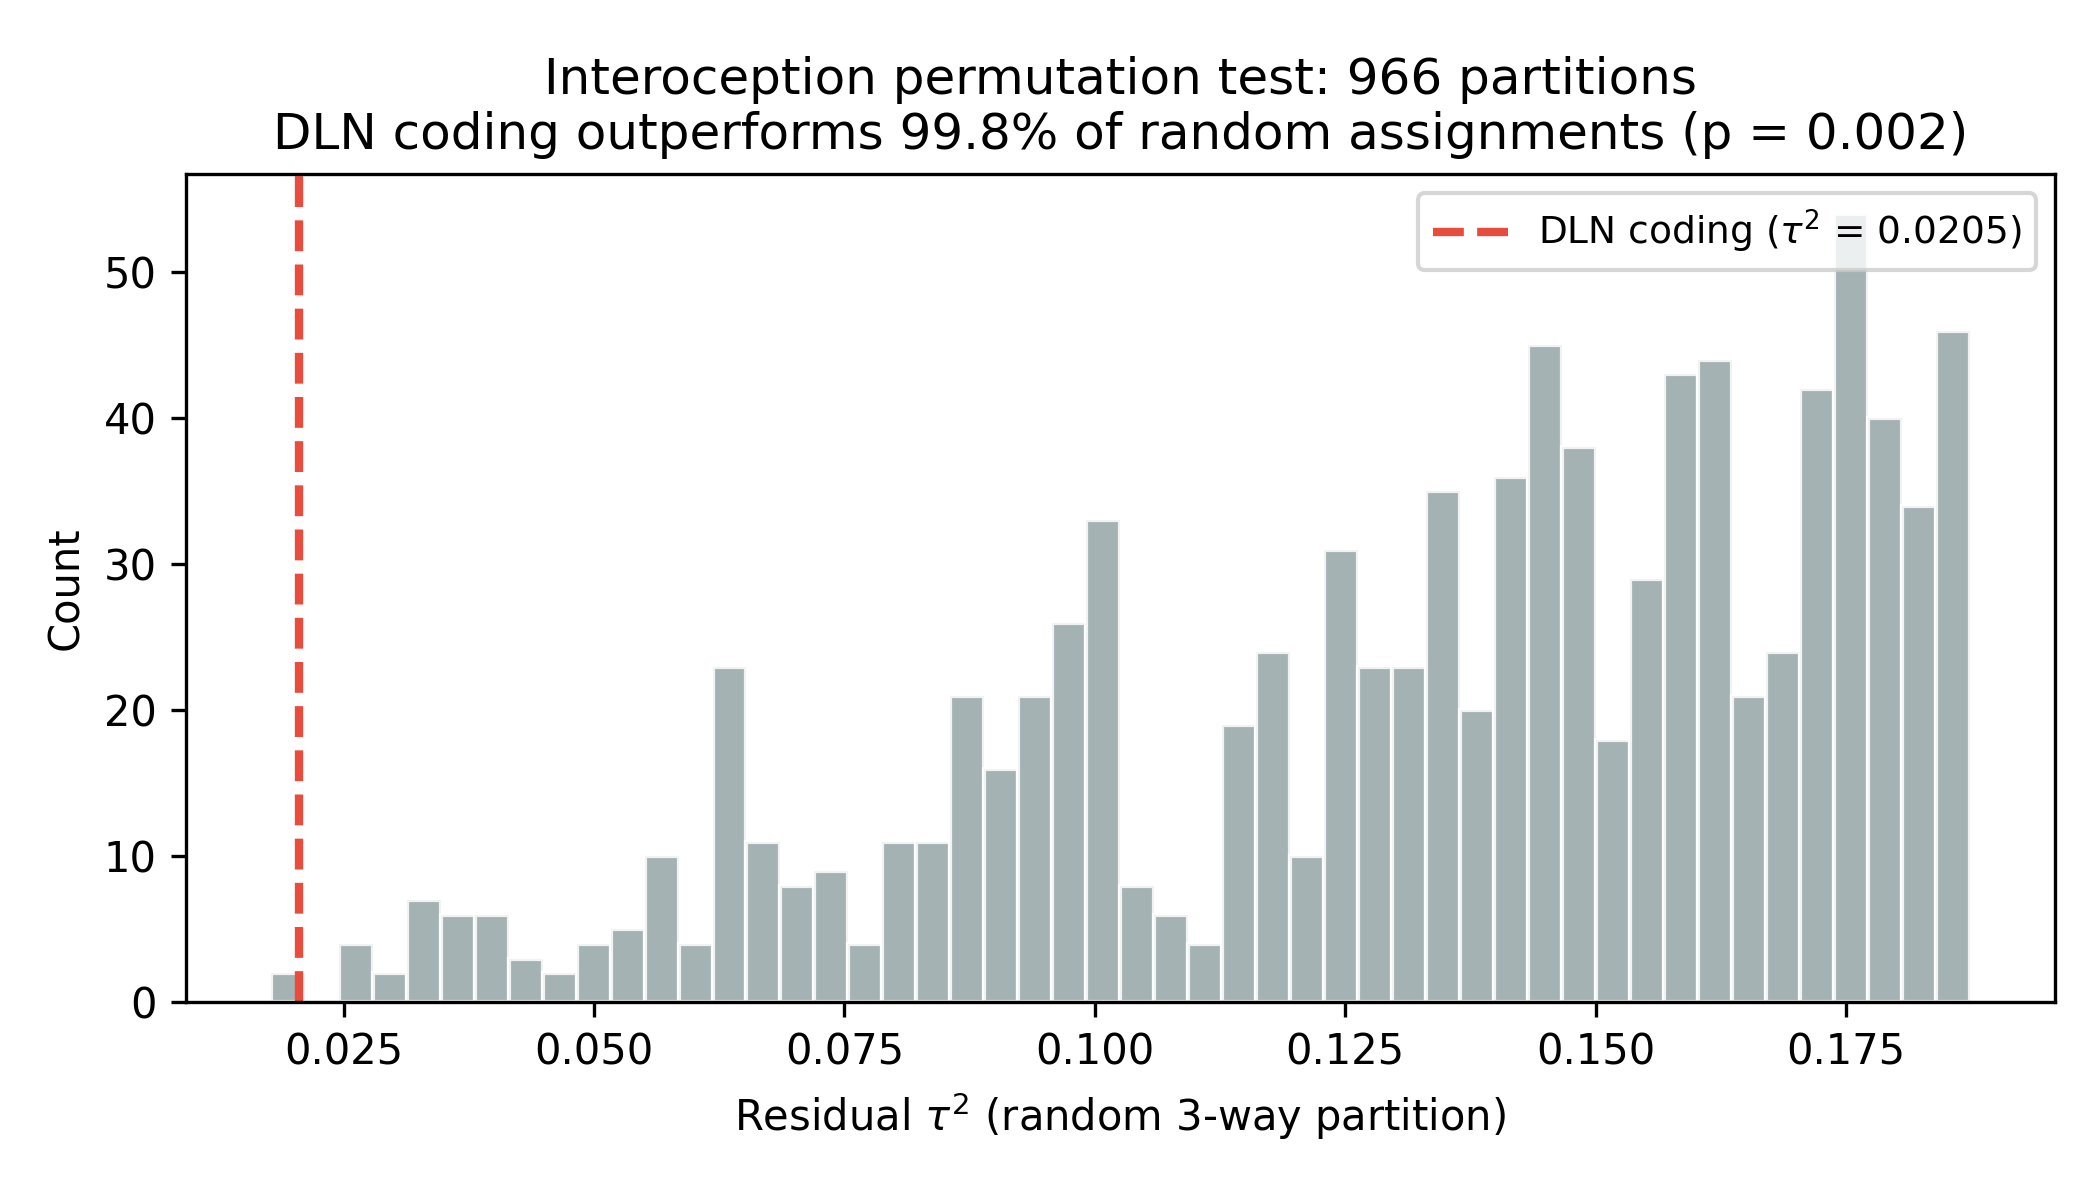
\includegraphics[width=0.48\linewidth]{../evidence_synthesis/outputs/figures/interoception_permutation_dist.png}%
\hfill
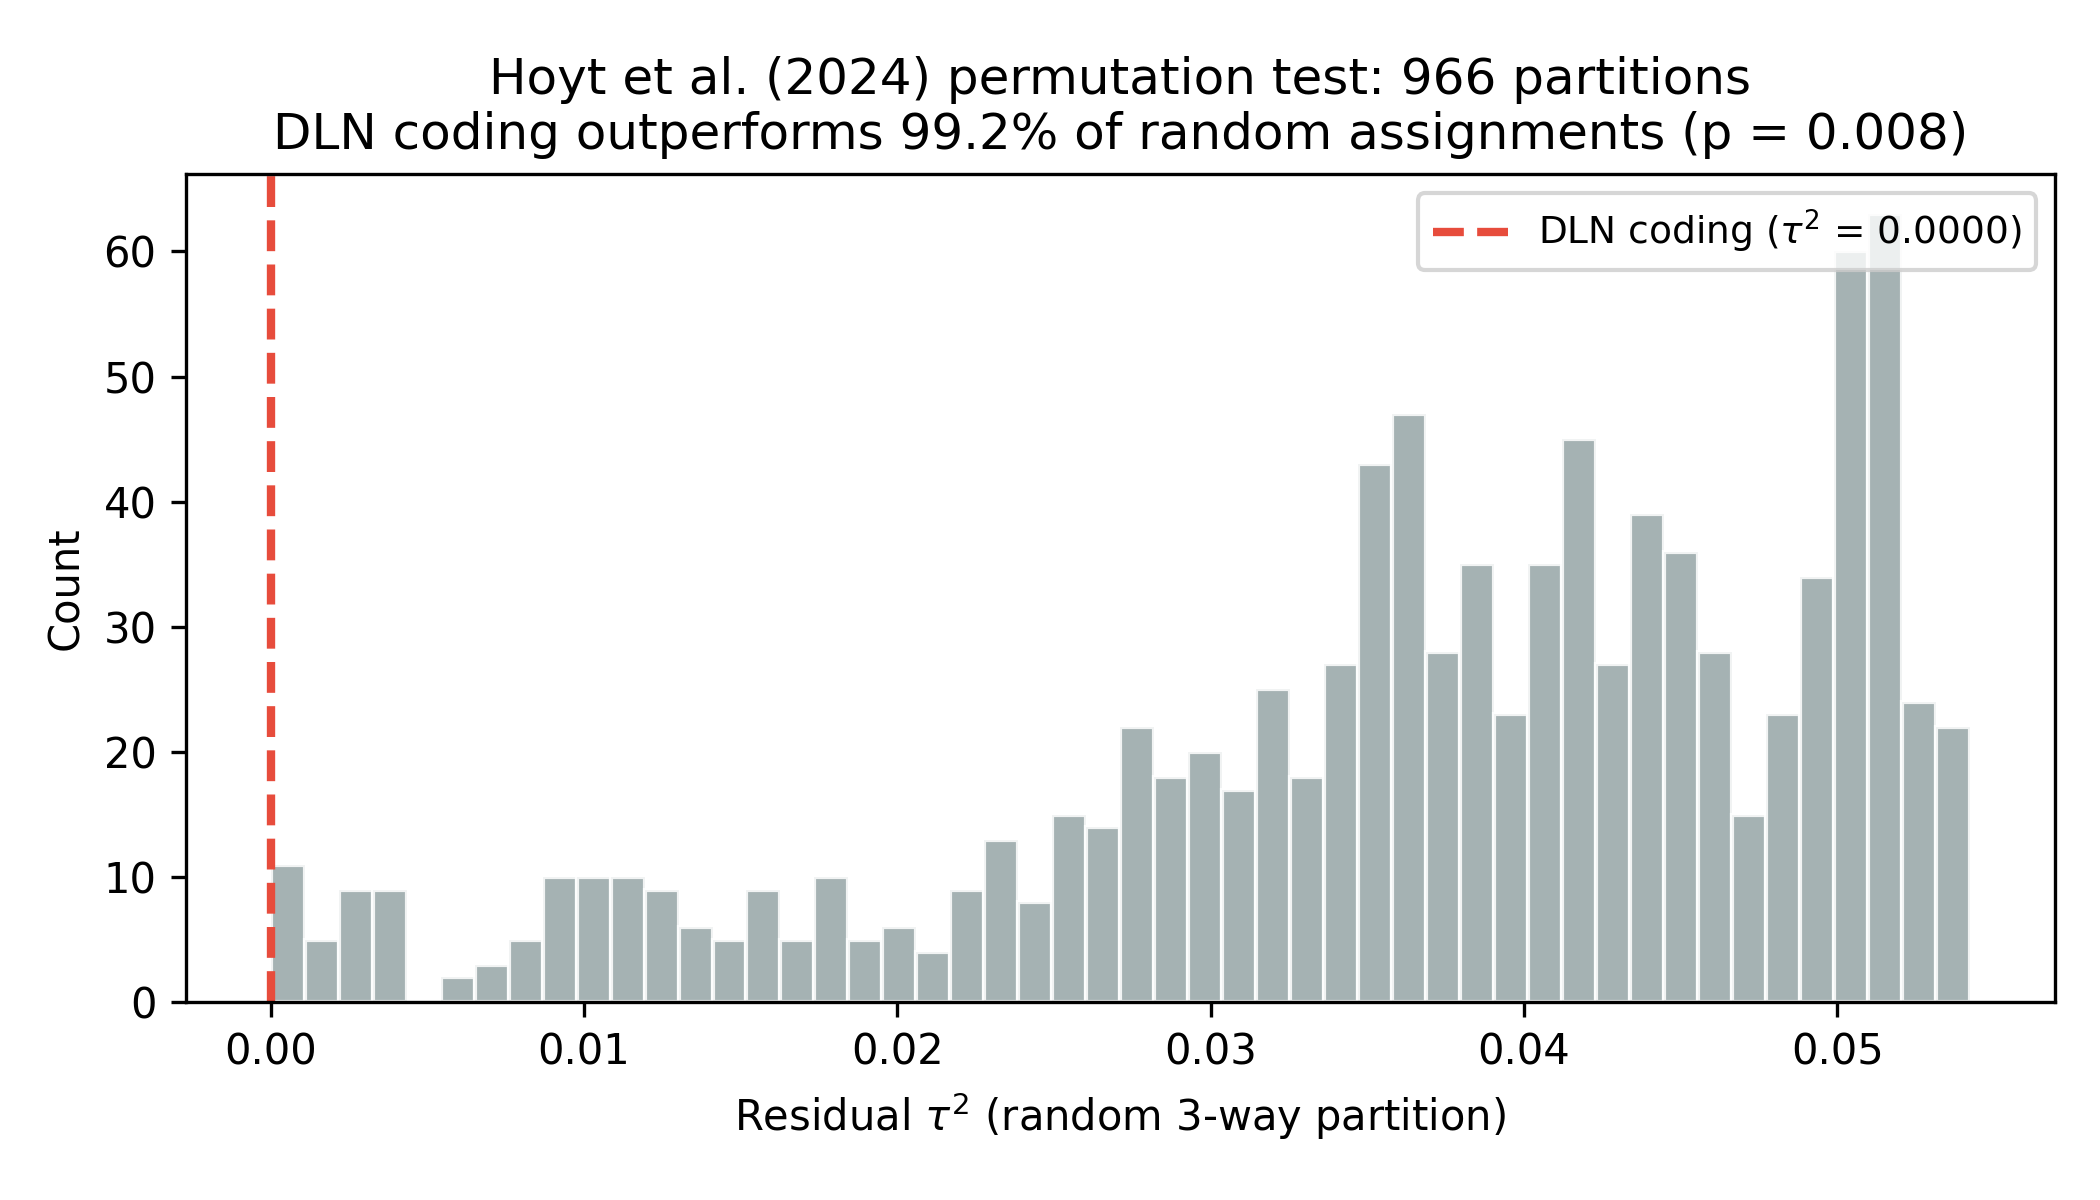
\includegraphics[width=0.48\linewidth]{../evidence_synthesis/outputs/figures/hoyt2024_permutation_dist.png}

\vspace{1em}

\centering
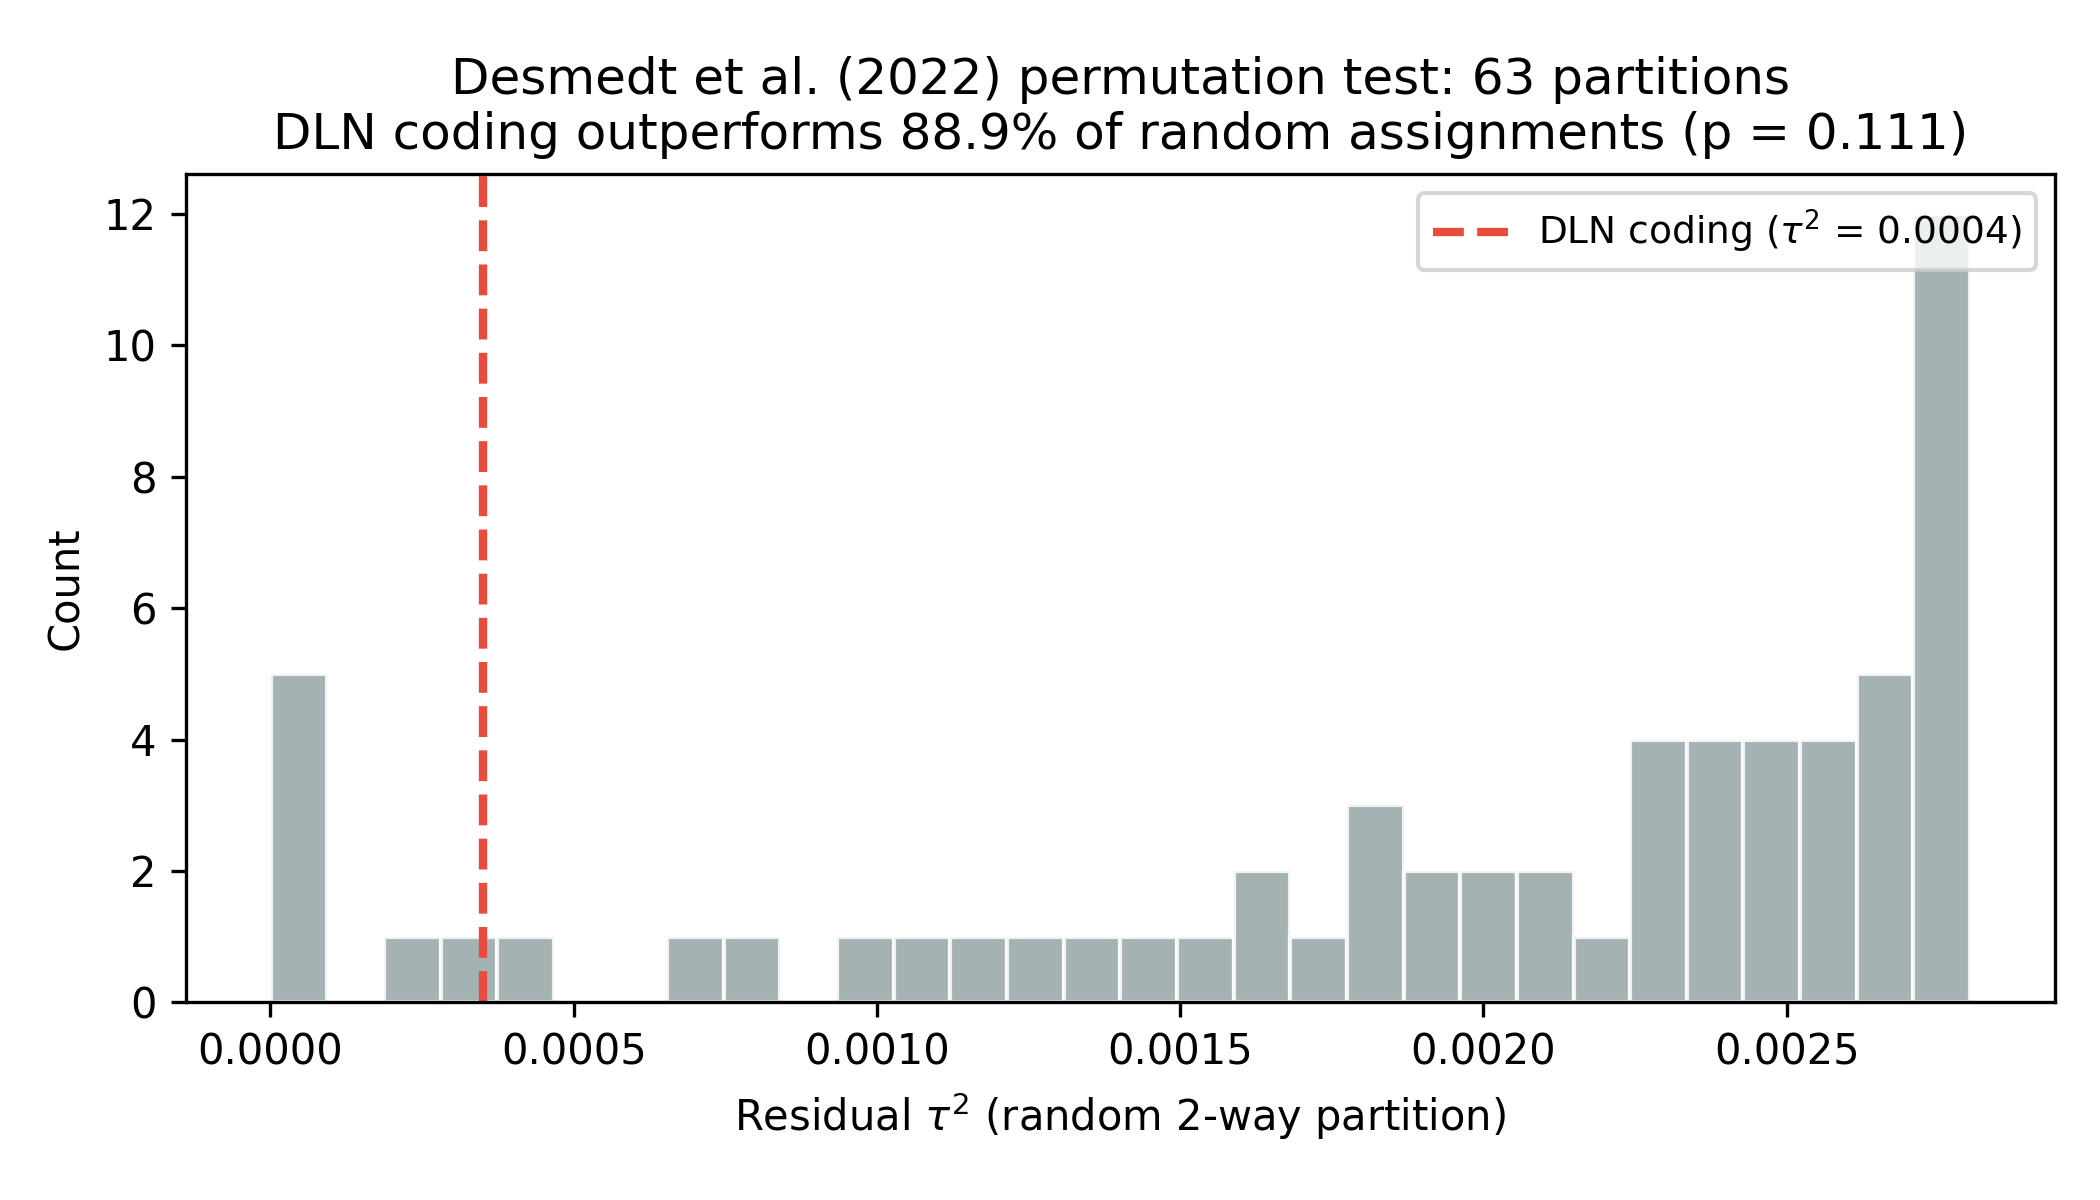
\includegraphics[width=0.48\linewidth]{../evidence_synthesis/outputs/figures/desmedt2022_permutation_dist.png}
\caption*{\textbf{Supplementary Figure 1.} Permutation distributions
for cross-domain datasets. \textbf{(a)}~Interoception--alexithymia
($k = 8$ measure families; $S(8,3) = 966$ partitions; $p = 0.002$):
DLN coding outperforms 99.8\% of random three-way assignments.
\textbf{(b)}~Emotional approach coping and health
(Hoyt et al., 2024; $k = 8$ outcome domains; $S(8,3) = 966$;
$p = 0.008$): DLN coding outperforms 99.2\% of random assignments.
\textbf{(c)}~Heartbeat counting task criterion validity
(Desmedt et al., 2022; $k = 7$ criteria; $S(7,2) = 63$ two-way
partitions; $p = 0.111$): DLN coding outperforms 88.9\% of random
assignments, though the test does not reach significance given limited
combinatorial resolution (minimum achievable $p = 1/63 \approx 0.016$).}
\end{figure}


\bibliography{references}

\end{document}
